\section{Nouvelles voies de formation avec $\mathrm{H}_2$ excité}

Dans certaines zones du nuage, une fraction importante de $\mathrm{H}_2$ est excitée par pompage UV dans ses états vibrationnels. Pour les réactions impliquant la molécule, une partie de l'énergie nécessaire à la réaction peut être prélevée dans son énergie interne ce qui a tendance à les favoriser. La prise en compte de l'énergie interne de la molécule a un impact sur les intensités des raies d'émissions de traceurs clés comme le $\mathrm{CO}$ \cite{COJoblin}, $\mathrm{H}_2$ ou $\mathrm{H}_2\mathrm{O}$. C'est un phénomène déjà bien connue pour la formation du $\mathrm{CH}^+$ (eq \ref{eq:C++H2}) \cite{Herraez, Zanchet}.

\begin{equation} \label{eq:C++H2}
    \begin{array}{lllclll}
        \mathrm{C}^+ & + &\mathrm{H}_2   & \rightarrow &\mathrm{CH}^+  & + & \mathrm{H} \\
    \end{array}
\end{equation}

Pour calculer le nouveau taux de réaction, le principe est de passer de la loi d'Arrhénius à un calcul des taux de réactions entre chaque populations des niveaux du $\mathrm{H}_2$ et de l'espèce $\mathrm{X}$. Cependant réaliser un calcul précis de ce phénomène est coûteux car il demande de connaître les taux de réactions d'une espèce avec la molécule $\mathrm{H}_2$ dans chacun de ses états excités. Afin de mieux expliquer les raies d'émissions, on cherche à comprendre comment un nouveau calcul des coefficients de réaction qui prend en compte l'énergie interne de $\mathrm{H}_2$ modifie les voies de formations des principaux traceurs. Sans connaître précisément les taux des réactions des populations de $\mathrm{H}_2$ avec 
des espèces autres que le $\mathrm{C}^+$, le code PDR fait une approximation de la nouvelle prescription. Si elle entraîne des changements majeurs dans la chimie et les raies d'émissions des traceurs, il sera alors intéressant de faire un calcul précis de ces taux. \newline 

Les différences les plus importantes que l'on observe sur les spectres d'émissions sont pour la molécule du $\mathrm{CO}$ (figure \ref{fig:type46:CO}), du $\mathrm{H}_2$ (figure \ref{fig:type46:H2}) et $\mathrm{H}_2\mathrm{O}$ (figure \ref{fig:type46:H2O}). Or, on sait jusqu'à présent que le $\mathrm{CO}$ est principalement formé à partir du $\mathrm{CH}^+$ et que le calcul précis du taux de formation du $\mathrm{CH}^+$ par le $\mathrm{C}^+$ (eq. \ref{eq:C++H2}) est déjà connu dans le code. L'analyse de la chimie montre que la voie de formation du $\mathrm{CO}$ par $\mathrm{OH}$ est devenue efficace ce qui contribue à former davantage de $\mathrm{CO}$ ($\times 10$) et à intensifier ses raies. Le schéma \ref{fig:type46:form:CO} rassemble les réactions servant à former la molécule. Par ailleurs, la découverte de cette nouvelle voie de formation par $\mathrm{OH}$ est un résultat important. 

\begin{figure}[!h]
    \centering 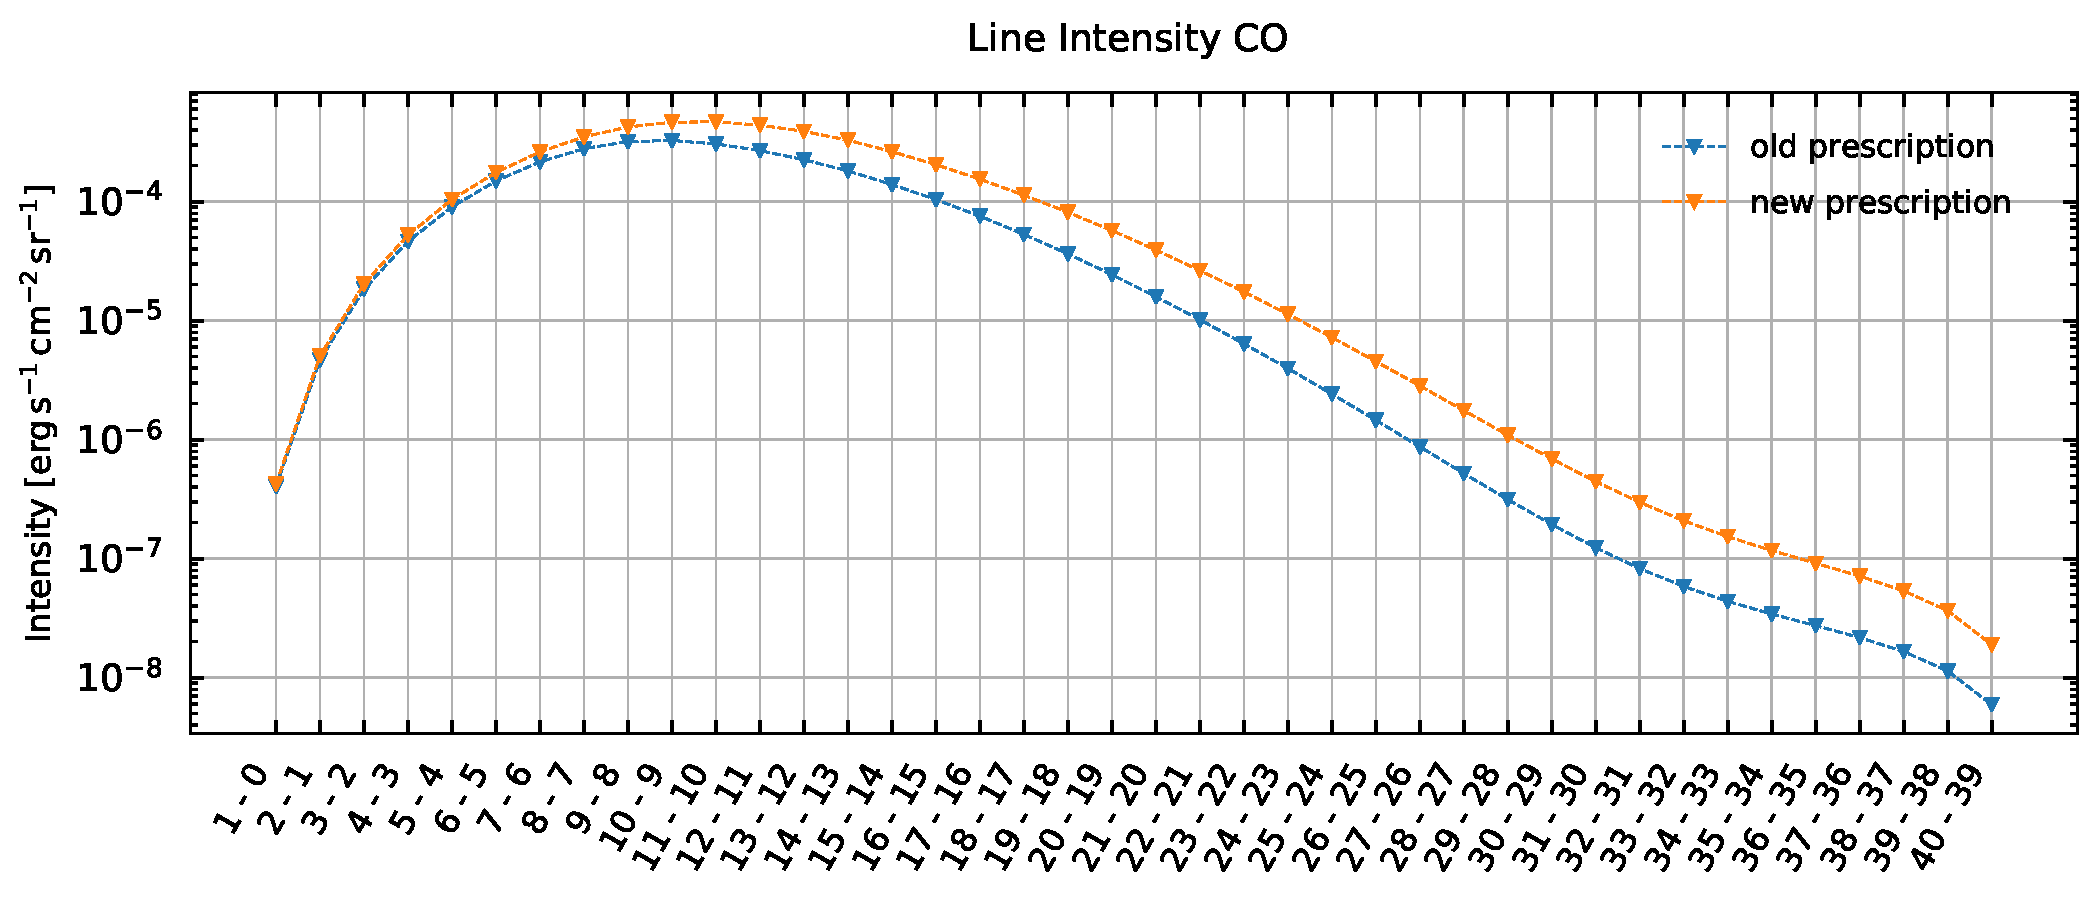
\includegraphics[trim = {0 0 0 1cm},clip,width=0.8\textwidth]{figure/type46/I_comp_CO.pdf}
    \caption{Diagramme d'excitation du $\mathrm{CO}$ avec la nouvelle prescription}
    \begin{minipage}{\textwidth}
    Seules les transitions rotationnelles du $\mathrm{CO}$ ont été écrites (toutes s'effectuent à $\mathrm{v}=0$). Un modèle isobare a été choisi ($\mathrm{P} = 2.8\,10^{8} \,\mathrm{cm}^3\,\mathrm{K}$ et $\chi = 3.1\, 10^4$).
    \end{minipage}
    \label{fig:type46:CO}
\end{figure}

\begin{figure}[!h]
    \centering \includegraphics[trim = {0 0 0 1cm},clip,width=0.8\textwidth]{}
    \caption{Réseau de formation du $\mathrm{CO}$}
    \begin{minipage}{\textwidth}
    
    \end{minipage}
    \label{fig:type46:form:CO}
\end{figure}

En comparant les réseaux chimiques du modèle avec la nouvelle prescription on trouve que la réaction $\mathrm{O} + \mathrm{H}_2 \rightarrow \mathrm{OH} +  \mathrm{H}$, devenue effiace, augmente la densité de $\mathrm{H}_2\mathrm{O}$ ($\times 10$) ainsi que ses raies d'émissions (figure \ref{fig:type46:H2O}). On constate également que la réaction $\mathrm{N} + \mathrm{H}_2 \rightarrow  \mathrm{NH} +  \mathrm{H}$ devient importante. La densité du $\mathrm{NH}$ augmente ($\times 10^3$) de même que celle du $\mathrm{HCN}$ ($\times 2$) et de $\mathrm{NO}$ ($\times 2$) <spectres du $\mathrm{NH}$ ?>. Il est présenté dans l'appendice \ref{} les voies de formations des espèces qui sont impactées par le nouveau calcul des taux de réactions.\newline 

Cette étude a notamment permis de découvrir une nouvelle voie de formation du $\mathrm{CO}$ et de déceler d'autres espèces susceptibles de réagir avec le $\mathrm{H}_2$ comme $\mathrm{N}$. Enfin, on a montré qu'une connaissance plus fine de la chimie impliquant la molécule $\mathrm{H}_2$ pouvait avoir un impact important sur les spectres d'émissions des traceurs comme le $\mathrm{CO}$. Il serait intéressant de continuer l'étude dans ce sens en comparant par exemple d'autres PDR avec des conditions physiques différentes.
